\section{Theoretical acoustic}\label{sec:section2}
%------------------------------------------------------------------------------------------------------------
%------------------------------------------------------------------------------------------------------------
%------------------------------------------------------------------------------------------------------------
%------------------------------------------------------------------------------------------------------------
\subsection{Acoustic in duct}
The acoustic in ducts is well-known and the main aspects were find by Helmholtz. A good overview can be found in this book \cite{Luck_thesis}.
We consider an infinite duct with x axis and a given section.

Acoustics is governed by few equations:
\begin{itemize}
    \item Mass continuity: 
        \begin{equation} 
        \frac{\partial \rho}{\partial t}+\mathrm{div}\rho v =0
        \end{equation}
    With $\rho$ the density, $v$ the velocity.
    \item Momentum continuity (given by the Navier-Stockes equation):
        \begin{equation} 
        \rho\frac{dv}{dt}=-\mathrm{grad} \rho+\mathrm{div} \tau+g
        \end{equation}
    \item energy continuity
\end{itemize}
However, these equations are too complex to be used analytically. Some assumptions are made:
\begin{itemize}
    \item Non-viscous fluid
    \item No thermal conductivity
    \item Entropy conservation
    \item Uniform mean flow
    \item Time dependence of $exp(iwt)$. The section is constant across the x axis. Thus $p\propto exp(iwt_\pm ikx)$
\end{itemize}
With the mass continuity and the momentum continuity, the convective Helmholtz equation can be found: 
    \begin{equation} 
    \Delta p +\Big[(w-ku_0)^2-k^2c_0^2\Big]p=0
    \end{equation}
With $\Delta$ the Laplace operator and $c$ the sound speed velocity.\\
The solution of this equations is a sum of different functions called modes: 
\begin{equation} 
    p(x,y,z,\omega)=\sum_{l=0}^\infty p_l^+ \Psi_l(y,z)e^{-ik_{x,l}(M,\omega)x}+p_l^- \Psi_l(y,z)e^{-ik_{x,l}(-M,\omega)x}
    \label{Convective_Helmholtz_Equation}
\end{equation}
With $M$ the mach number $M={v}/{c}$. The $l$ modes are sorted by frequency. Each mode has an acoustic shape in the section $(y,z)$. The mode can propagate in two different directions, in the positive or the negative direction.
The usual problem in acoustic is the significant number of modes which are not negligible. In the duct, only few modes propagate unattenuated. Indeed, over a certain cut-off frequency $Re(k_{x,l})$ is negative, these modes are attenuated quickly. This cut-off frequency depends of the geometry and the mach number. For usual duct, just one mode propagates energy, the plane wave mode.
%------------------------------------------------------------------------------------------------------------
\subsubsection{Rectangular duct} \label{sec:RectDuct}
To solve Eq.\eqref{Convective_Helmholtz_Equation}, the separation of variables method is used. The mode shapes are independent between the directions y and z (called $m$ modes for y direction and $n$ for z). For rigid wall boundary conditions:
\begin{equation} 
    \Psi_{m,n}(y,z)=\Psi_{m}(y)\Psi_{n}(z)=\cos(\frac{m\pi y}{2b})\cos(\frac{n\pi z}{2h})
\end{equation}
With $b$ and $h$ the width and the height.
The axial wave number $k_{x,(m,n)}$ is solution of the dispersion equation: 
\begin{equation} 
    k_{x,(m,n)}=k_0\frac{M\pm\sqrt{1-(1-M^2)\Big[(\frac{m\pi}{2ka})^2+(\frac{n\pi}{2kh})^2\Big]}}{1-M^2}
\end{equation}
Mode will propagate if:
\begin{equation} 
    k\geq\sqrt{(1-M^2)\Big[(\frac{m\pi}{2a})^2+(\frac{n\pi}{2h})^2\Big]}
\end{equation}
The transverses waves numbers respect: 
\begin{equation} 
    k_{y,(m)}=\frac{m\pi}{2a} \ \text{and} \ k_{z,(n)}=\frac{n\pi}{2h}
\end{equation}
\begin{figure}[H] \centering
    \begin{subfigure}{.5\textwidth}\centering
     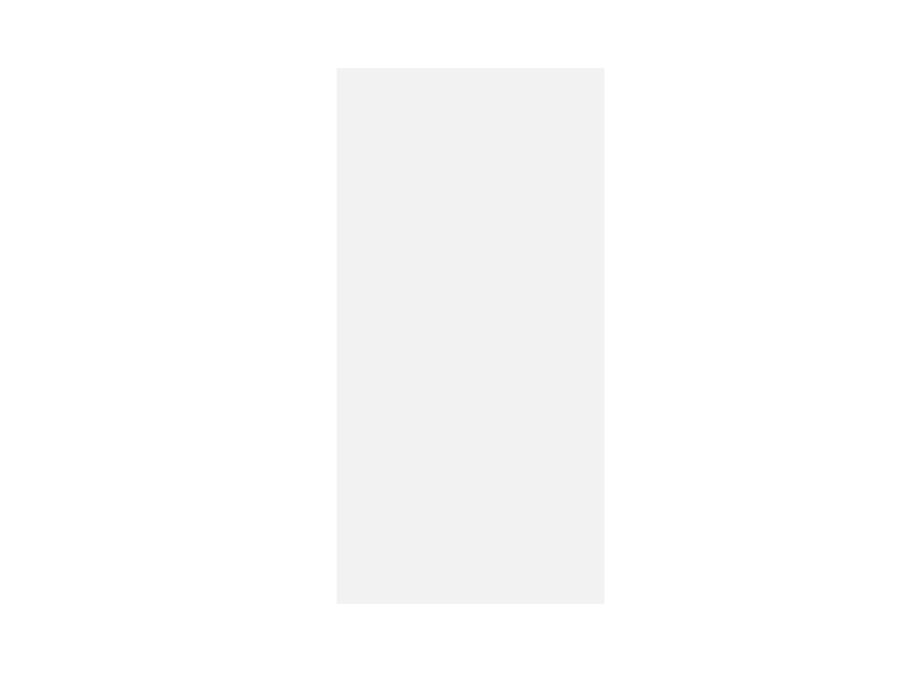
\includegraphics[width=.8\linewidth]{modeR00}
     \caption{(0,0) plane wave mode}
    \end{subfigure}%
    \begin{subfigure}{.5\textwidth}\centering
     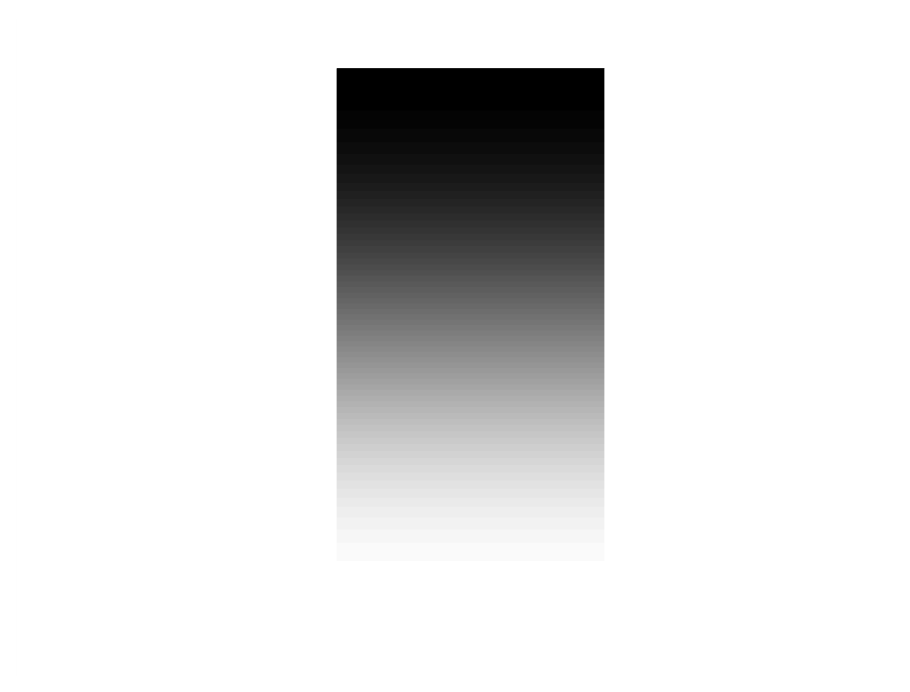
\includegraphics[width=.8\linewidth]{modeR01}
     \caption{(0,1)}
    \end{subfigure}\\
    \begin{subfigure}{.5\textwidth}\centering
     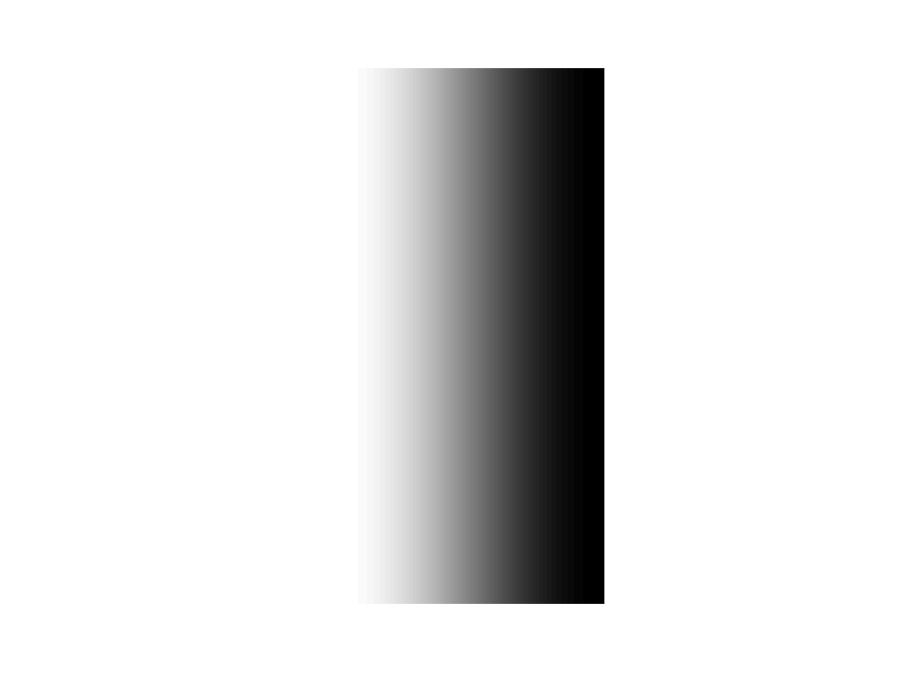
\includegraphics[width=.8\linewidth]{modeR10}
     \caption{(1,0)}
    \end{subfigure}%
    \begin{subfigure}{.5\textwidth}\centering
     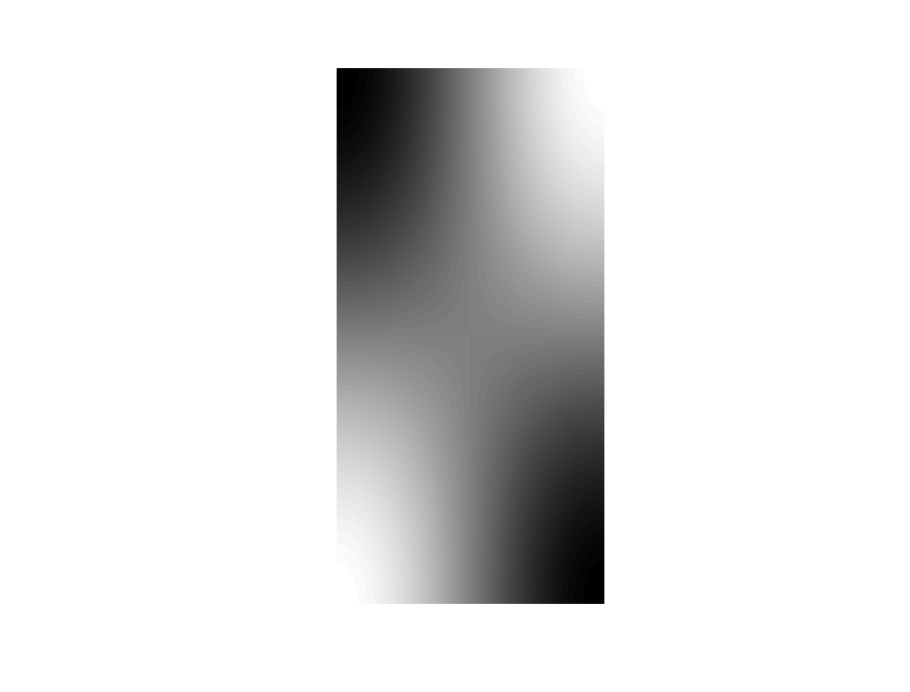
\includegraphics[width=.8\linewidth]{modeR11}
     \caption{(1,1)}
    \end{subfigure}
    \caption{Mode shape (m,n) in a rectangular duct}
\end{figure}
%------------------------------------------------------------------------------------------------------------
\subsubsection{Circular duct}
The radius is called R ($0<r<R$).
For circular duct, there are two kinds of modes: \textbf{circumferential and radial modes (called respectively $m$ and $n$)}. The mode shape is not independent between the radial and circumferential direction. 
\begin{equation} 
    \Psi_{m,n}(r,\theta)=J_m(k_{r,(m,n)} r)e^{jm\theta}
\end{equation}
Where $k_{r,(m,n)}=\frac{j_{mn}}{R}$. $J_m$ is the Bessel function and $j_{mn}$ is the n-th zero of $J_m^'$:
\begin{equation} 
    J_m^'(j_{mn})=0
\end{equation}
The axial wave number $k_{x,(m,n)}$ respect the dispersion equation: 
\begin{equation} 
    k_{x,(m,n)}=k_0\frac{M\pm\sqrt{1-(1-M^2)(\frac{j_{mn}}{kR})^2}}{1-M^2}
\end{equation}
Mode will propagate if:
\begin{equation} 
    kR\geq j_{mn}\sqrt{1-M^2}
\end{equation}
The radial wave number is: 
\begin{equation} 
    k_{r,(m,n)}=\frac{j_{mn}}{R}
\end{equation}
\begin{figure}[H] \centering
    \begin{subfigure}{.5\textwidth}\centering
     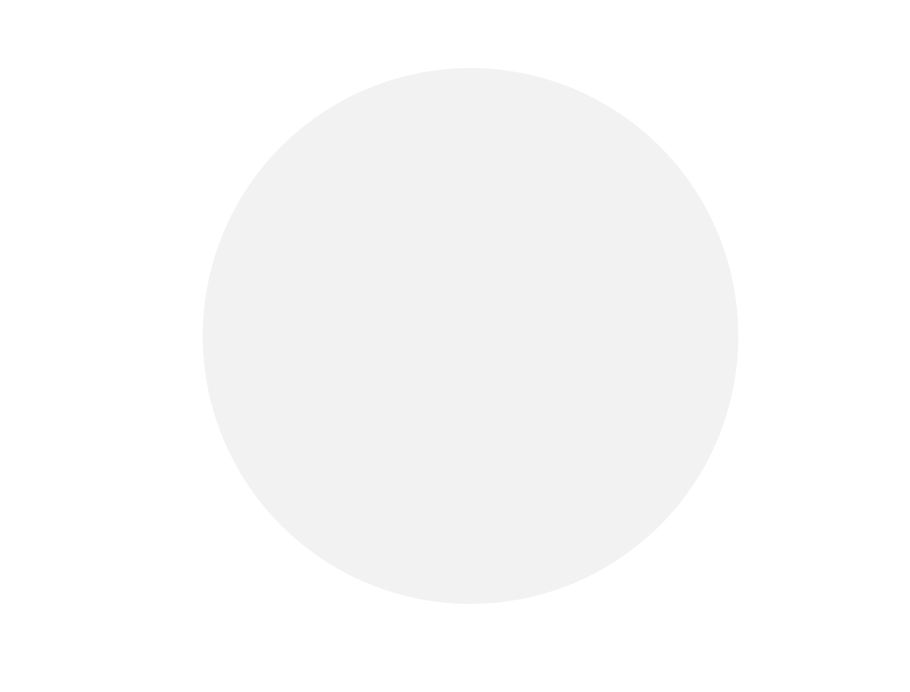
\includegraphics[width=.8\linewidth]{modeC00}
     \caption{(0,0) plane wave mode}
    \end{subfigure}%
    \begin{subfigure}{.5\textwidth}\centering
     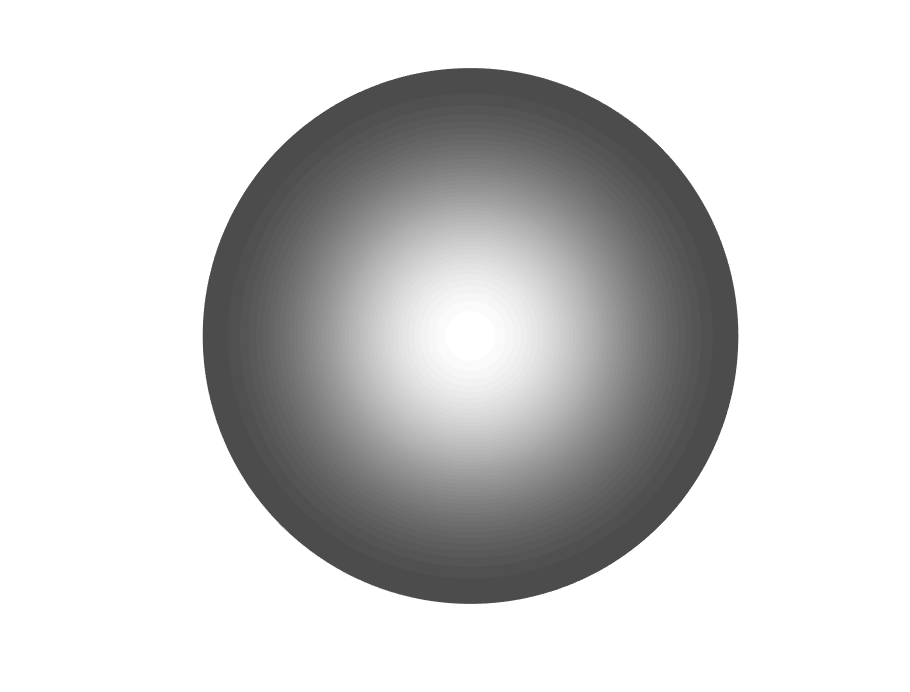
\includegraphics[width=.8\linewidth]{modeC01}
     \caption{(0,1)}
    \end{subfigure}\\
    \begin{subfigure}{.5\textwidth}\centering
     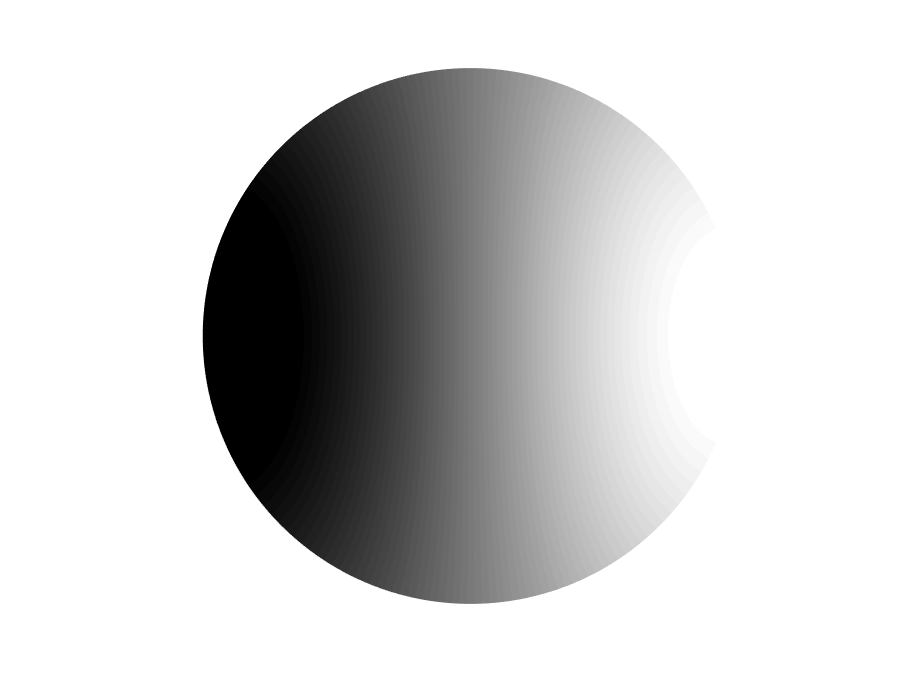
\includegraphics[width=.8\linewidth]{modeC10}
     \caption{(1,0)}
    \end{subfigure}%
    \begin{subfigure}{.5\textwidth}\centering
     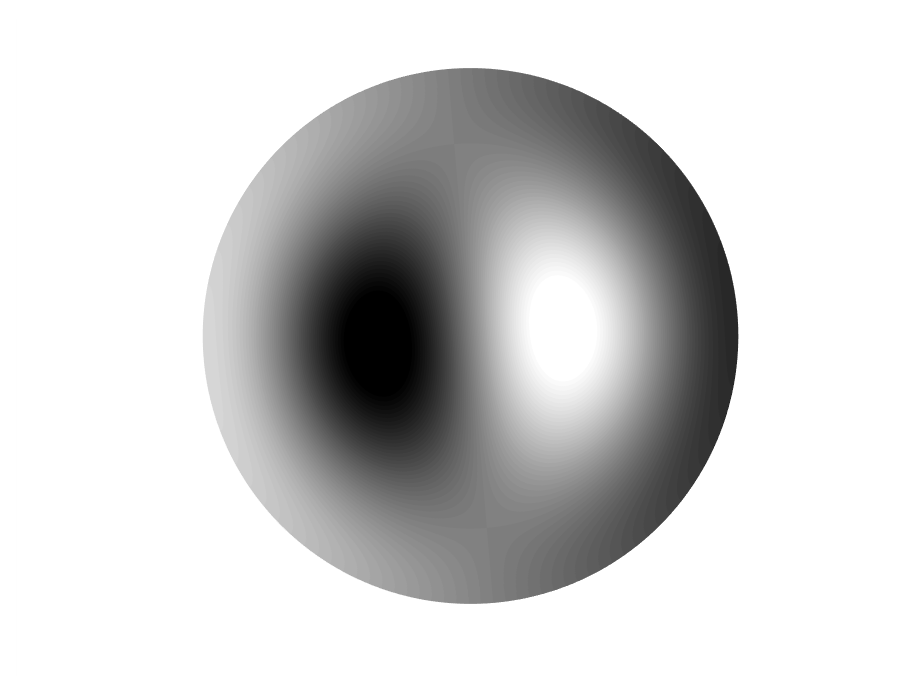
\includegraphics[width=.8\linewidth]{modeC11}
     \caption{(1,1)}
    \end{subfigure}
    \caption{Mode shape in a circular duct}
\end{figure}
%------------------------------------------------------------------------------------------------------------
\subsubsection{Wall attenuation}
\textbf{Model of attenuation}\\
The viscosity is not negligible at the interface wall/flow. A model of attenuation given by Pierce \cite{Pierce} is:
\begin{equation} 
    k=\frac{\omega}{c}+(1+i)\frac{1}{2\sqrt{2}}\sqrt{\frac{\omega\mu}{\rho c^2}}\Bigg[1+\frac{\gamma -1}{\sqrt{Pr}}\Bigg]\frac{L_p}{A}
\end{equation}
$Pr$ is the Prandtl number, $\rho$ the density, $L_p$ the perimeter and $A$ the area. An easy way to use attenuation is to replace $k_0=k$\smallbreak
\noindent\textbf{Boundary condition: Ingard-Myers}\\
For a wall of impedance Z, the boundary condition is still in discussion. Ingard assumes the continuity of acoustic particle displacement with uniform flow \cite{Ingard}. Myers extend the model for non-uniform mean-flow \cite{Myers}:
\begin{equation} 
    \label{eq:Myers}
    \frac{\partial p}{\partial z}|_{wall}=\frac{ik}{Z}(1-iM\frac{\partial}{\partial x})^2 p|_{wall}
\end{equation}
%------------------------------------------------------------------------------------------------------------
%------------------------------------------------------------------------------------------------------------
%------------------------------------------------------------------------------------------------------------
%------------------------------------------------------------------------------------------------------------
\subsection{Scattering matrix}
The scattering matrix is a very powerful tool in the duct acoustic field. The applications are very different and the scattering matrix is also available for N-ports. To assess the acoustic properties of a liner, a lined section is placed between two hard duct wall: 
\begin{figure}[H] \centering
    \label{Scatteringmatrix}
    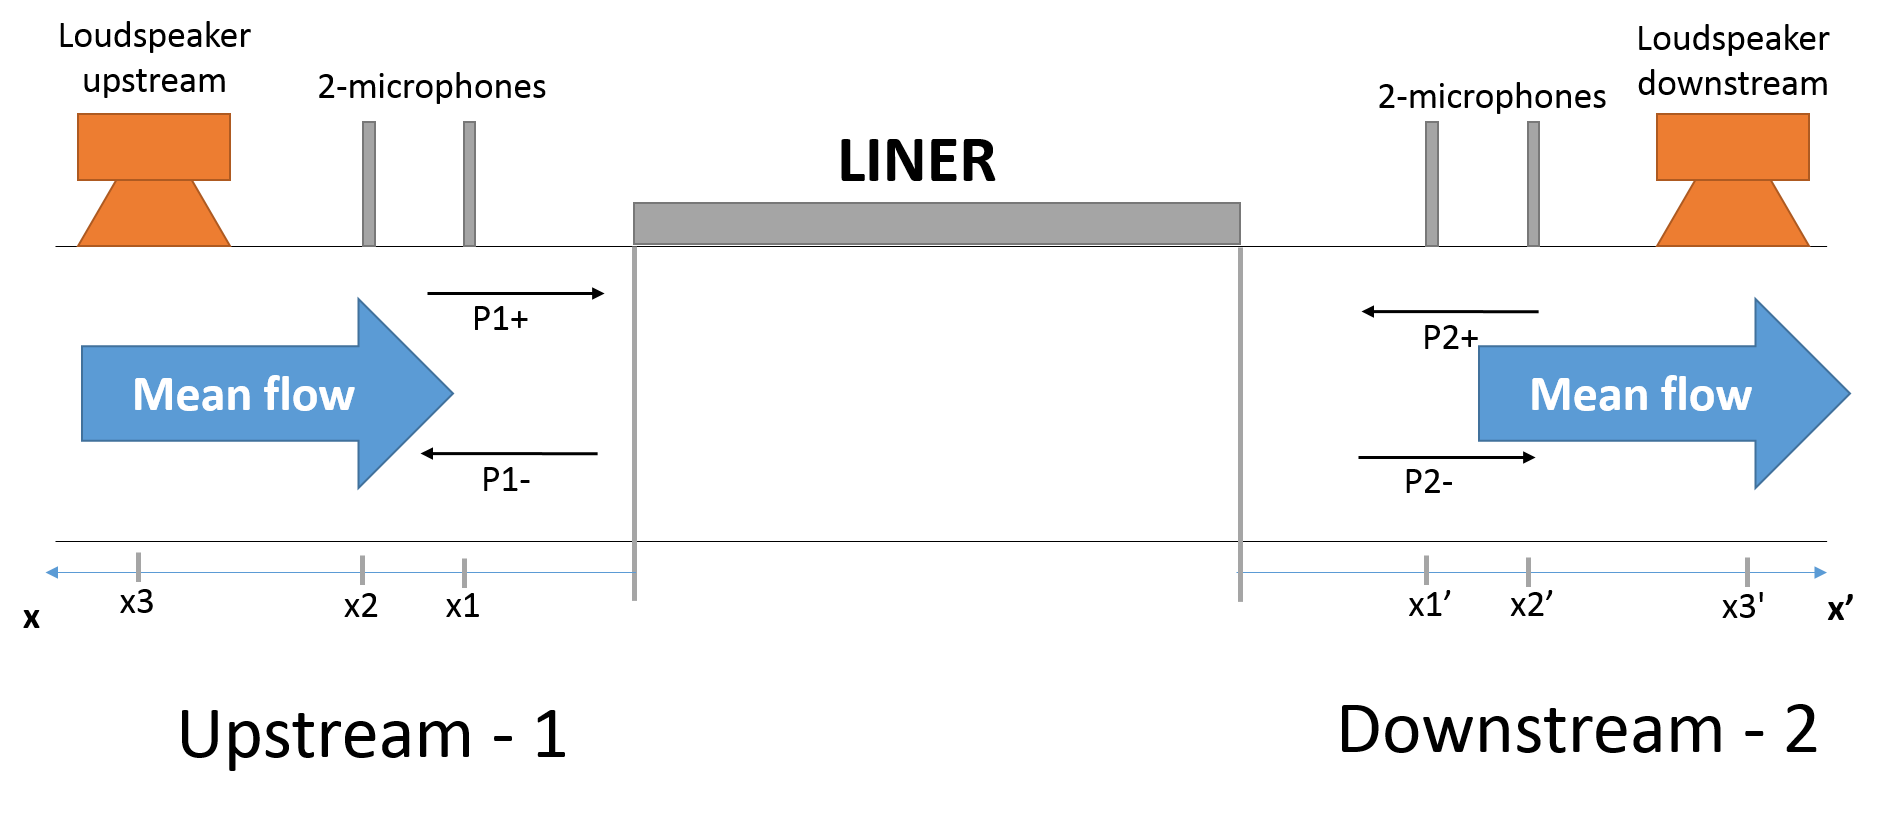
\includegraphics[scale=0.45]{Scatteringmatrix}
    \caption{Scattering matrix setup}
\end{figure}
The excitation is one time at the upstream and one other time at the downstream. The properties are not equals for the downstream and the upstream because of the presence of a flow. The usual notation is $p^+$ for the wave which moves towards the lined section and $p^-$ for the waves which moves off.
The reflection and transmission coefficients are determined:
\begin{equation}
    p^-=Sp^+
\end{equation}
\begin{gather}
    S=
    \begin{pmatrix}
      R_{11} & T_{21} \\
      T_{12} & R_{22} 
    \end{pmatrix}
\end{gather}
\begin{gather}
    \begin{pmatrix}
      p_1^- \\
      p_2^- 
    \end{pmatrix}
    =
    \begin{pmatrix}
      R_{11} & T_{21} \\
      T_{12} & R_{22} 
    \end{pmatrix}
    \begin{pmatrix}
      p_1^+ \\
      p_2^+ 
    \end{pmatrix}
 \end{gather}
 
However the pressures $p_+$ and $p_-$ have to be preliminary determined. The well-known method of two-microphones is an easy way to do the wave decomposition \cite{Boden_2micros}.  
For each measurement and for each side, two microphones measure the pressure $p_1$ and $p_2$. 
The following system gives the pressures $p_+$ and $p_-$ for the upstream \textbf{or} downstream case.
\begin{gather}
    \begin{pmatrix}
      e^{ik_x^-x_1} & e^{-ik_x^+x_1} \\
      e^{ik_x^-x_2} & e^{-ik_x^+x_2}
    \end{pmatrix}
    \begin{pmatrix}
       p^-\\
       p^+
    \end{pmatrix}
    =
    \begin{pmatrix}
      p_1 \\
      p_2 
    \end{pmatrix}
 \end{gather}
It's possible to use more than 2 microphones, the system is over-determined.
 \begin{gather}
    \begin{pmatrix}
      e^{ik_x^-x_1} & e^{-ik_x^+x_1} \\
      \vdots & \vdots\\
      e^{ik_x^-x_i} & e^{-ik_x^+x_i}\\
      \vdots & \vdots\\
      e^{ik_x^-x_n} & e^{-ik_x^+x_n}
    \end{pmatrix}
    \begin{pmatrix}
       p^-\\
       p^+
    \end{pmatrix}
    =
    \begin{pmatrix}
      p_1 \\
      \vdots\\
      p_i \\
      \vdots\\
      p_n
    \end{pmatrix}
 \end{gather}
 There is lot of discussion about the combination of microphones which has to be used to get the more accurate decomposition.\\
 \\
To simplify the notations, since the beginning the pressure $p$ was the complex pressure $\hat{p}$:
\begin{equation}
    \hat{p}(\omega)=P(\omega)e^{i\phi(\omega))}
\end{equation}
Where $P$ is the amplitude and $\phi$ the phase (the reference is the source).\smallbreak
There are different methods to get this complex pressure. We used the Hilbert transform:
\begin{equation}
    \widetilde{x}(t)=x(t)+i\ \textbf{Hilbert}[x(t)]=X(t)e^{i\psi(t))}
\end{equation}
Where $\psi(t)$ is the instantaneous phase and $X(t)$ the temporal envelop of the signal. The instantaneous pulsation is:
\begin{equation}
    \omega=\frac{d\psi}{dt}
\end{equation}
For $\tau$ multiple of half of the excitation frequency, the true transfer function between the source and the microphone is:
\begin{equation}
    H=\frac{2}{\tau}\int_0^{\tau}\! \frac{y(t)}{\widetilde{r}(t)} \, dt 
\end{equation}
%------------------------------------------------------------------------------------------------------------
%------------------------------------------------------------------------------------------------------------
%------------------------------------------------------------------------------------------------------------
%------------------------------------------------------------------------------------------------------------
\subsection{Impedance acoustic}
There are several methods to determine the acoustic impedance. In this master thesis the single mode straightforward method and the mode matching method are implemented.
%------------------------------------------------------------------------------------------------------------
%------------------------------------------------------------------------------------------------------------
\subsubsection{Impedance tube measurement}
The older way to measure the impedance is the impedance tube measurement. A loudspeaker and the liner are mounted on the pipe extremities.
\begin{figure}[H] \centering
    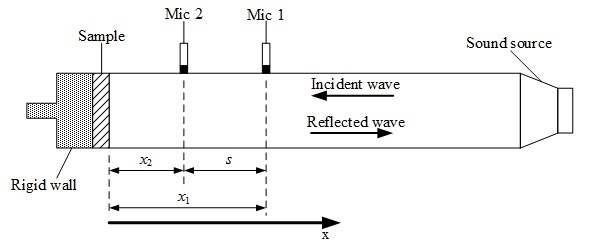
\includegraphics[scale=0.8]{Impedance_Tube}
    \caption{Impedance tube}
\end{figure}
The acoustic field is composed by stationary waves. The distance between two successive nodes can be measured and gives the impedance. This measure is not accurate. A more accurate measurement can be obtained thanks to a wave decomposition with the 2-microphones method. $p^+$ and $p^-$ are determine and the impedance is given by \cite{Absorption_Coefficients_and_Impedance}: 
\begin{equation}
    Z(w)=\rho cS\Bigg[\frac{p^++p^-}{p^+-p^-}\Bigg]
\end{equation}
%------------------------------------------------------------------------------------------------------------
%------------------------------------------------------------------------------------------------------------
\subsubsection{The in-situ method}
It is assumed that there is only the plane wave mode inside the cavity.
The methods is describes in this paper \cite{Boden_method}. One microphone measure the pressure field $p_s$ flush with the liner surface. A second one is inside the cavity (height $h$) and measures $p_c$. The transfer function between the two microphones gives the impedance:
\begin{equation}
    Z(w)=-i\frac{H_{cs}}{\sin(kh)}
\end{equation}
The acoustic field measured is the close one. It's possible to move the first microphone to reduce the impact of the closed field:
\begin{figure}[H] \centering
    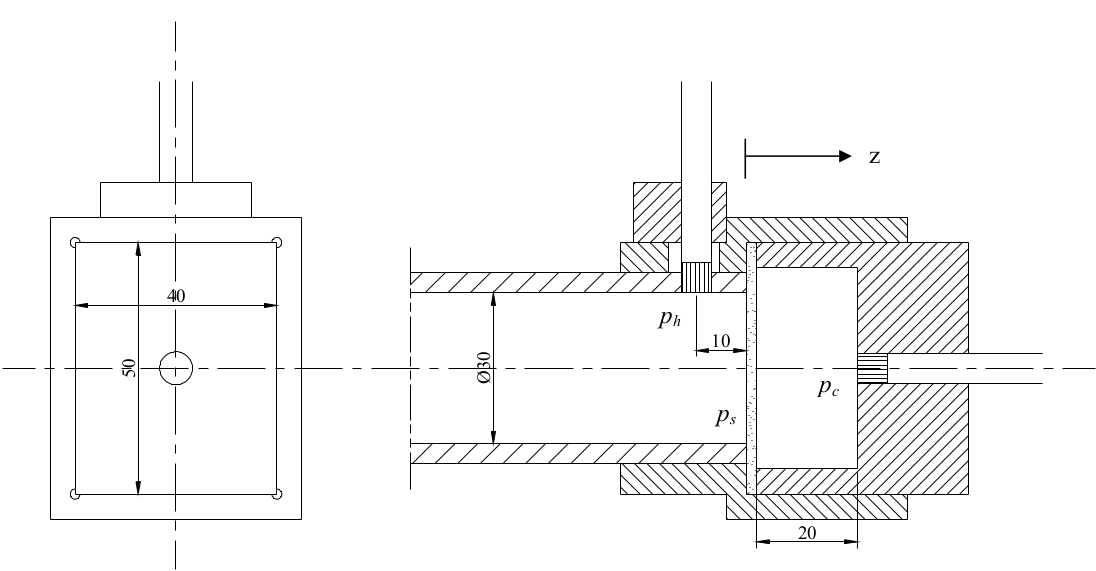
\includegraphics[scale=0.35]{In_situ}
    \caption{The in-situ method}
\end{figure}
%------------------------------------------------------------------------------------------------------------
%------------------------------------------------------------------------------------------------------------
\subsubsection{The mode matching method}
The mode matching method is a well-known method. The modes shapes have to be determined before. Each steps of the determination of these modes is in \nameref{sec:EigenvalueRect}. The geometry is: 
\begin{figure}[H] \centering
    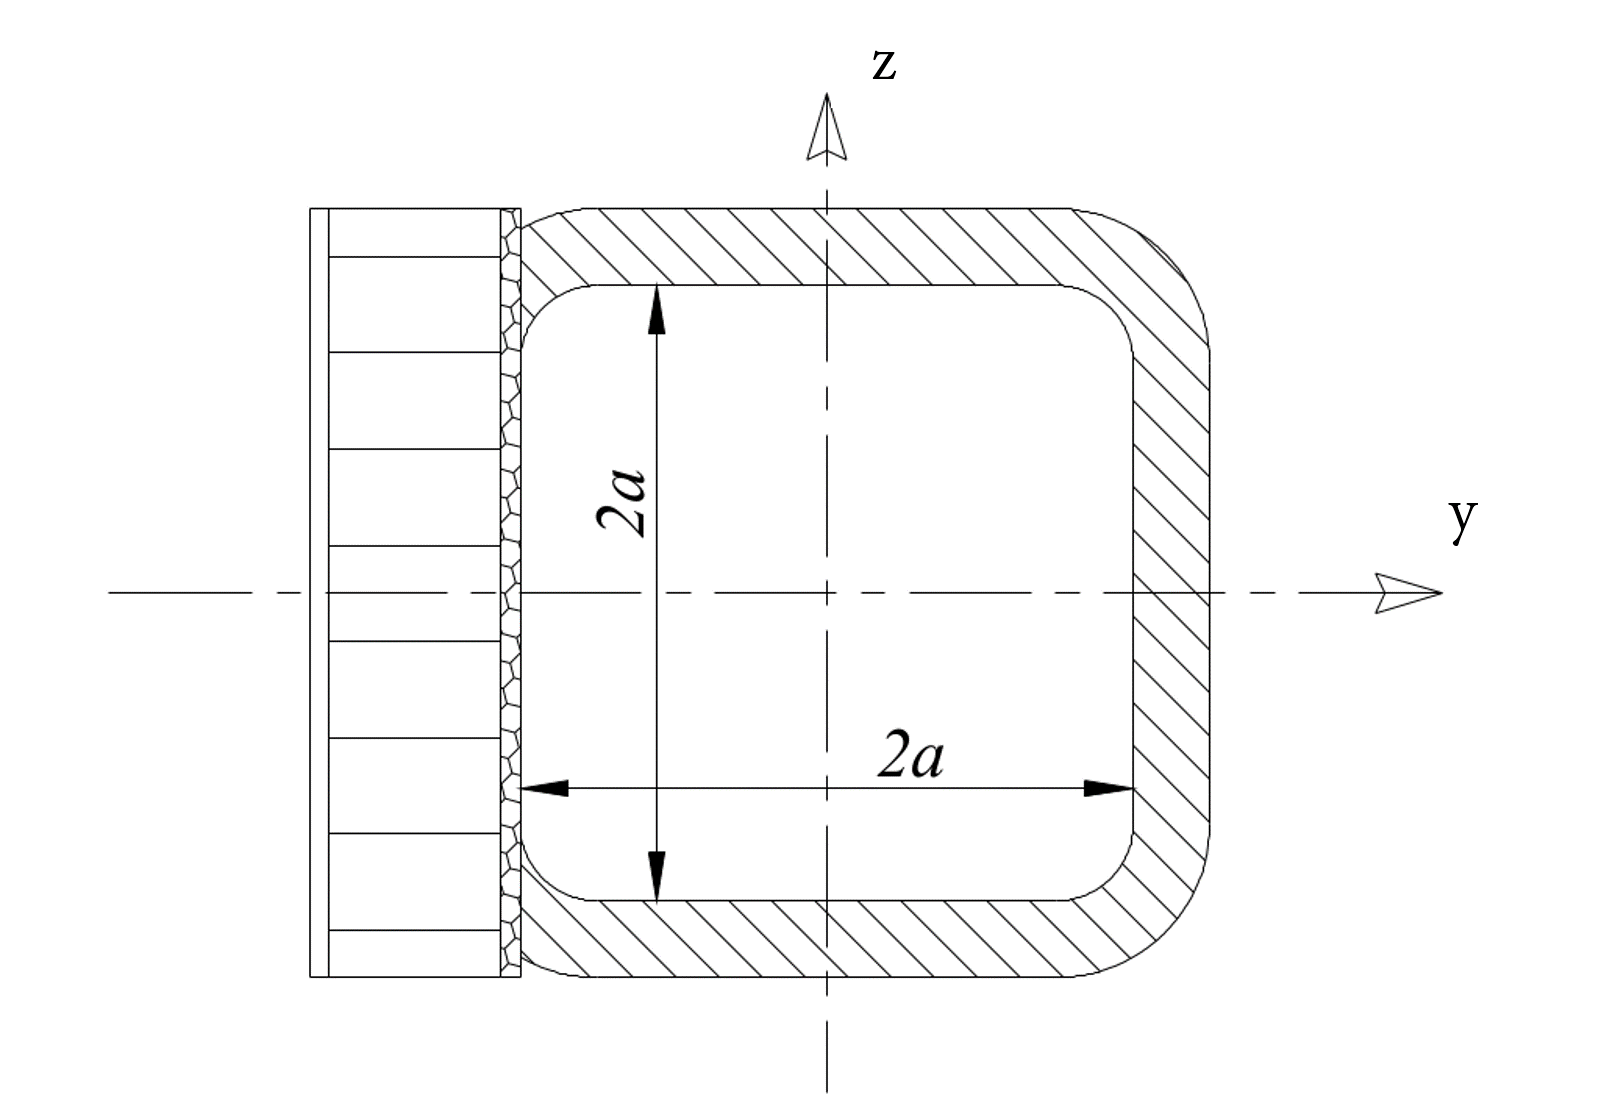
\includegraphics[scale=0.25]{Zhourectduct}
    \caption{Rectangular duct lined for y=-a}
\end{figure}
\noindent Note that the coordinates are different from \ref{sec:RectDuct} \nameref{sec:RectDuct}.\\
The incident wave is a plan wave, the direction y and z are independent. For the z direction, the boundary conditions are hard walls, the solutions are orthogonal. Thus there is just the $n=0$ mode in the z direction. For the y direction the modes of the lined wall are not orthogonal, higher mode $m$ will appear. The problem is reduced to a 2 dimensions probelm $(x,y)$.
The rig is decomposed in three parts:
\begin{figure}[H] \centering
    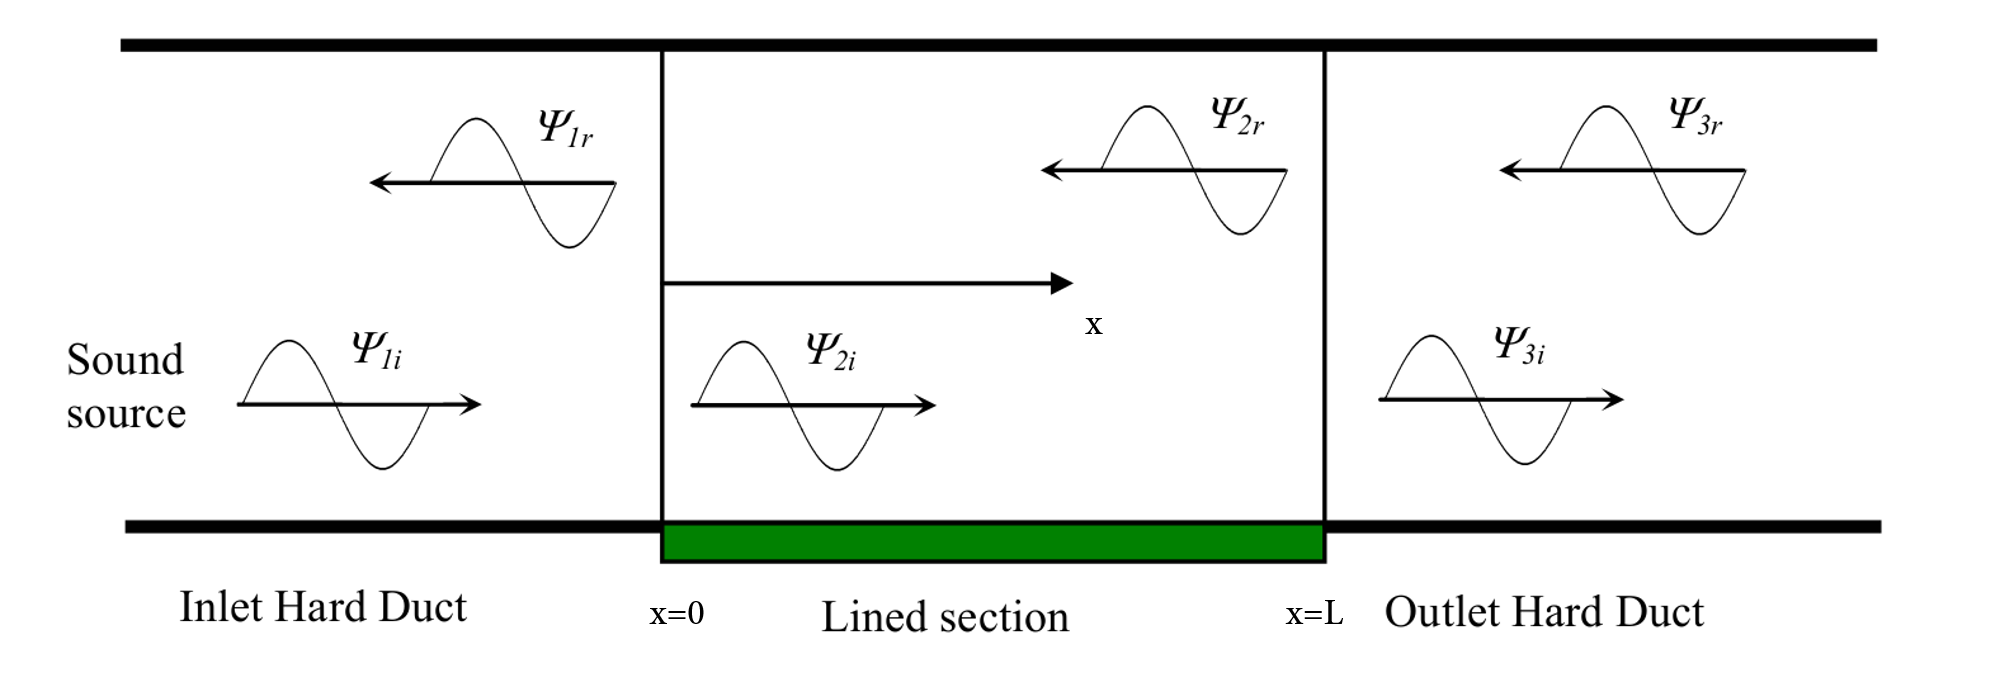
\includegraphics[scale=0.4]{ModeMatch}
    \caption{Coordinates for mode-matching }
\end{figure}
The pressures are given by:
\begin{itemize}
    \item for the upstream hard section:
    \begin{equation}
        p_1(x,y)=a_1^+ \Psi_{1i,1}(y)e^{-ik_{x1i,1}x}+\sum_{m=0}^\infty a_m^- \Psi_{1r,m}(y)e^{ik_{x1r,m}x}
    \end{equation}
    With $\Psi_{1i,m}(y)=\Psi_{1r,m}(y)$: 
    \begin{equation}
        \left\{
        \begin{array}{ll}
         \Psi_{1,m}(y)=2\cos(\frac{m\pi}{2a}y)\ \text{for} \ n=2p \\
        \\
        \Psi_{1,m}(y)=2i\sin(\frac{m\pi}{2a}y) \ \text{for} \ n=2p+1
       \end{array}
       \right.
    \end{equation}
    \item for lined section (one wall lined at the opposite of a hard wall):
    \begin{equation}
        p_2(x,y)=\sum_{m=0}^\infty b_m^+ \Psi_{2i,m}(y)e^{-ik_{x2i,m}x}+\sum_{m=0}^\infty b_m^- \Psi_{2r,m}(y)e^{ik_{x2r,m}(x-L)}
    \end{equation}
    With: 
    \begin{equation}
        \Psi_{2i,m}(y)=e^{ik_{y2i,m}y}-e^{-ik_{y2i,m}(y-2a)}
    \end{equation}
    \item for the downstream hard section:
    \begin{equation}
        p_3(x,y)=\sum_{m=0}^\infty c_m^+ \Psi_{3i,m}(y)e^{-ik_{x3i,m}(x-L)}+c_1^- \Psi_{3r,1}(y)e^{ik_{x3r,1}(x-L)}
    \end{equation}
    With $\Psi_{3i,m}(y)=\Psi_{3r,m}(y)$:   
    \begin{equation}
        \left\{
        \begin{array}{ll}
         \Psi_{3,m}(y)=2\cos(\frac{m\pi}{2a}y)\ \text{for} \ m=2p \\
        \\
        \Psi_{3,m}(y)=2i\sin(\frac{m\pi}{2a}y) \ \text{for} \ m=2p+1
       \end{array}
       \right.
    \end{equation}
\end{itemize}
For the following part, the Mach number is considered zero to simplify the equation. Mode-matching with mean flow can be found here \cite{ModematchM}.
At each interface the pressure and the velocity are continuous:
\begin{equation}
    p_1(0,y)=p_2(0,y)
\end{equation}
and
\begin{equation}
    p_2(L,y)=p_3(L,y)
\end{equation}
\begin{equation}
    \frac{\partial p_1}{\partial x}\Bigg|_{x=0}=\frac{\partial p_2}{\partial x}\Bigg|_{x=0}
\end{equation}
and
\begin{equation}
    \frac{\partial p_2}{\partial x}\Bigg|_{x=L}=\frac{\partial p_3}{\partial x}\Bigg|_{x=L}
\end{equation}
By now the notation $k_{...,m}=k_{...}^{(m)}$ is used.
Multiplied by $\Psi_1^{(u)}$ where u=0..M, and integrated over the cross-section: 
\begin{equation}
    \sum_{m=0}^{M-1} a_m^-\Lambda_{11}^{mu}-\sum_{m=0}^{M-1} b_m^+\Lambda_{2i1}^{mu}-\sum_{m=0}^{M-1} b_m^-\Lambda_{2r1}^{mu}e^{-ik_{x2r}^{(m)}L}=-a_1^+\Lambda_{11}^{1u}
\end{equation}
\begin{equation}
    \sum_{m=0}^{M-1} c_m^+\Lambda_{11}^{mu}[1+R_e]-\sum_{m=0}^{M-1} b_m^+\Lambda_{2i1}^{mu}e^{-ik_{x2i}^{(m)}L}-\sum_{m=0}^{M-1} b_m^-\Lambda_{2r1}^{mu}=0
\end{equation}
\begin{equation}
    -\sum_{m=0}^{M-1} a_m^-\Lambda_{11}^{mu}k_{x1r}^{(m)}-\sum_{m=0}^{M-1} b_m^+\Lambda_{2i1}^{mu}k_{x2i}^{(m)}+\sum_{m=0}^{M-1} b_m^-\Lambda_{2r1}^{mu}k_{x2r}^{(m)}e^{-ik_{x2r(m)}L}=-a_1^+\Lambda_{11}^{1u}k_{x1i}^{(1)}
\end{equation}
\begin{equation}
    \sum_{m=0}^{M-1} c_m^+\Lambda_{11}^{mu}(k_{x3i}^{(m)}-R_ek_{x3r(m)})-\sum_{m=0}^{M-1} b_m^+\Lambda_{2i1}^{mu}k_{x2i}^{(m)}e^{-ik_{x2i}^{(m)}L}+\sum_{m=0}^{M-1} b_m^-\Lambda_{2r1}^{mu}k_{x2r}^{(m)}e^{-ik_{x2r}^{(m)}L}=0
\end{equation}
With $R_e$ the reflection coefficient at the end of the duct and the index:
\begin{equation}
    \Lambda_{pv}^{mu}=\iint \limits_S \Psi_p^{(m)} \Psi_v^{(u)} ds
\end{equation}
The true relations are for $M=\infty$. However the Index showed that the amplitudes of the higher modes quickly decrease. To avoid too much computation time, only the first modes are computed.\\
The system can be reduce to the following matrix:
\begin{gather} 
    \begin{bmatrix}
       \Lambda_{11}^{mu} & 0 & -\Lambda_{2i1}^{mu} & -\Lambda_{2ri1}^{mu}e^{-ik_{x2r}^{(m)}L} \\
       \\
      0 & \Lambda_{11}^{mu}[1+R_e] & -\Lambda_{2i1}^{mu}e^{-ik_{x2i}^{(m)}L} & -\Lambda_{2r1}^{mu}\\
      \\
      -\Lambda_{11}^{mu}k_{x1r}^{(m)} & 0 & -\Lambda_{2i1}^{mu}k_{x2i}^{(m)} & -\Lambda_{2ri1}^{mu} k_{x2r}^{(m)} e^{-ik_{x2r}^{(m)}L}\\
      \\
      0 & \Lambda_{11}^{mu}[k_{x3i}^{(m)}-R_ek_{x3r}^{(m)}]  & -\Lambda_{2i1}^{mu}k_{x2i}^{(m)}e^{-ik_{x2i}^{(m)}L} & \Lambda_{2ri1}^{mu} k_{x2r}^{(m)}
    \end{bmatrix}
    \begin{bmatrix}
       a_m^-\\
       \\
       c_m^+\\
       \\
       b_m^+\\
       \\
       b_m^-\\
       \\
    \end{bmatrix}
    \\
    =
    \begin{bmatrix}
        -a_1^+\Lambda_{11}^{1u}\\
       \\
       0\\
       \\
       -a_1^+\Lambda_{11}^{1u}k_{x1i}^{(1)}\\
       \\
       0\\
       \\
    \end{bmatrix}
\end{gather}
With $\Lambda_{pv}^{mu}$ a $M*M$ matrix. The index can be analytically calculated \cite{ModematchM}.\\
The system has 4M unknowns. To solve it, $a_1^+$ and $Re$ have to be measured. The two-microphones methods can be used in the upstream and downstream section.
%------------------------------------------------------------------------------------------------------------
%------------------------------------------------------------------------------------------------------------
\subsubsection{The single mode straightforward method}
This method is a simplified problem of the mode matching technique.
For the the single mode straightforward method, it assumes that only the first mode exist in the lined section \cite{Zhou_thesis}. The amplitudes of the higher modes are considered negligible (for low frequency). Moreover if it assumes that there is just an incident wave ($b_{(1)}^-=0$ and $c_{(1)}^-=0$). With these assumptions:
\begin{equation}
    k_{x2i}^{(1)}=\frac{i\ln\Big(\frac{\tau_{13}}{1+R_{11}}\Big)}{L}\ , \ k_{x2r}^{(1)}=\frac{i\ln\Big(\frac{\tau_{31}}{1+R_{33}}\Big)}{L}
\end{equation}
The impedance is given by \ref{eq:Impedance}
\clearpage
%------------------------------------------------------------------------------------------------------------
%------------------------------------------------------------------------------------------------------------
%------------------------------------------------------------------------------------------------------------
%------------------------------------------------------------------------------------------------------------
\subsection{Optimum Cremer impedance}
The problems consists to attenuate a specific mode. The problem is asymmetric with a locally reacting impedance, the boundary conditions are the Ingard-Myers conditions.
The general dispersion relationship for a circular and annular duct:
\begin{equation} 
    k_{x,(m,n)}=k_0\frac{M\pm\sqrt{1-(1-M^2)\Big(\frac{k_{r,(mn)}}{R}\Big)^2}}{1-M^2}
\end{equation}
The axial wave number depends only on the radial wave number. And with an impedance wall, the radial wave numbers are wander into their quarter of the complex plane in a irregular way. 
\begin{figure}[H] \centering
    \begin{subfigure}{.5\textwidth}\centering
     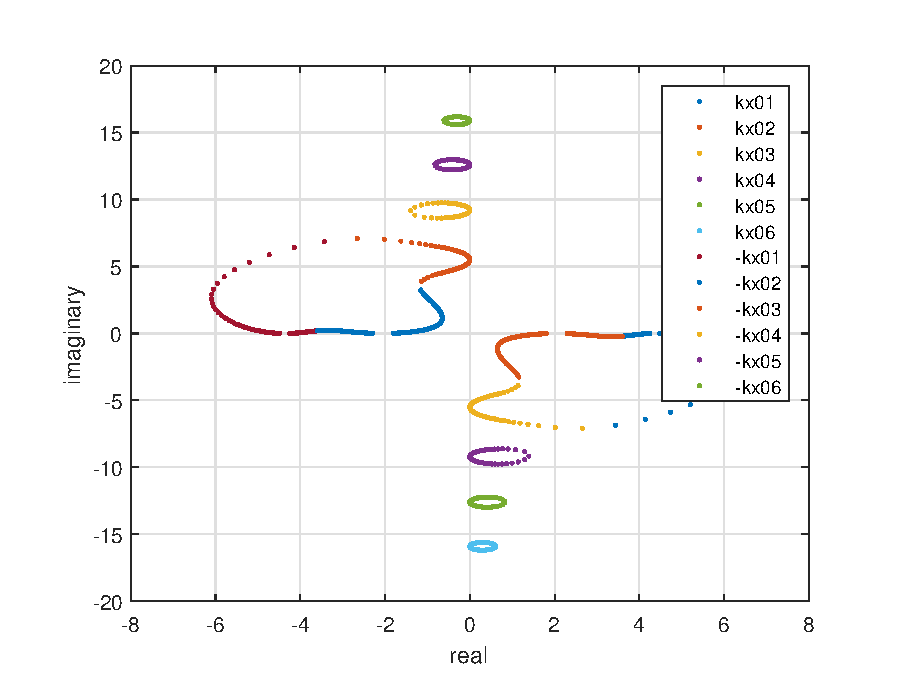
\includegraphics[width=1.13\linewidth]{kx01_05}
     \caption{$real(Z)=0.5$ and $im(Z)=-\infty \ to +\infty$}
    \end{subfigure}%
    \begin{subfigure}{.5\textwidth}\centering
     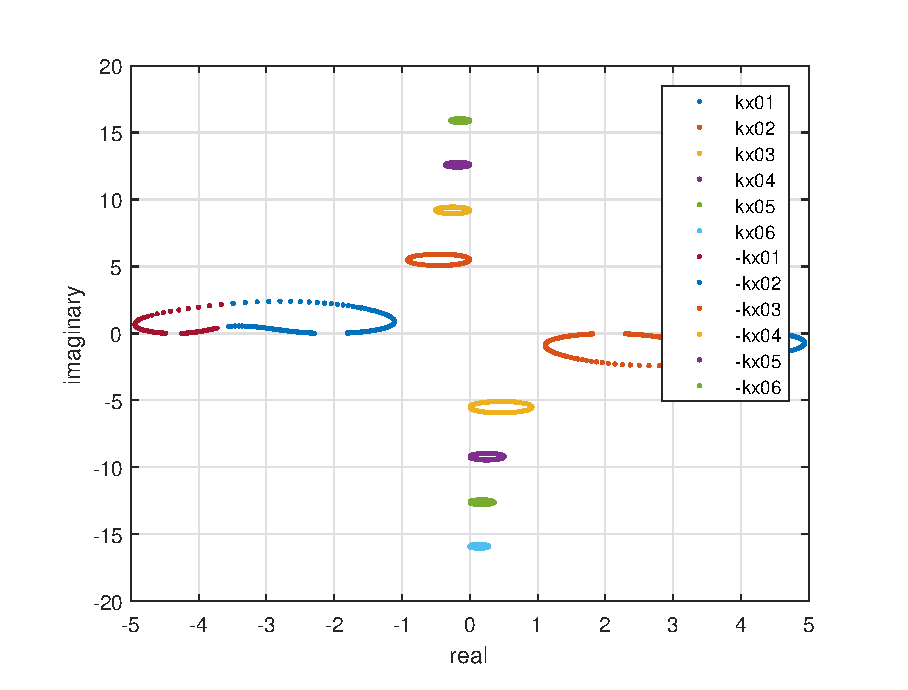
\includegraphics[width=1.13\linewidth]{kx01_10}
     \caption{$real(Z)=1$ and $im(Z)=-\infty \ to +\infty$}
    \end{subfigure}\\
    \begin{subfigure}{.5\textwidth}\centering
     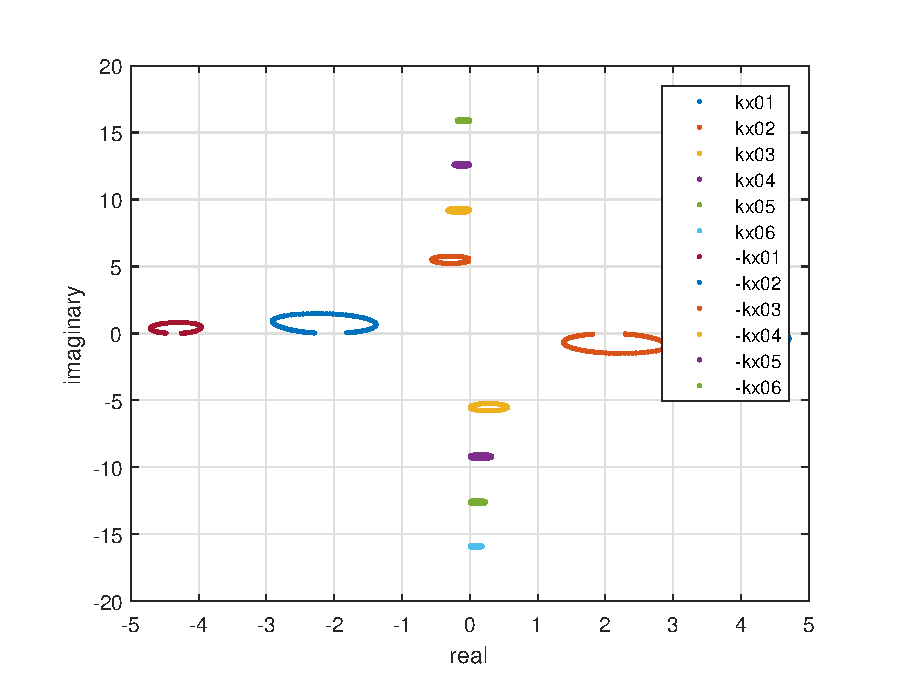
\includegraphics[width=1.13\linewidth]{kx01_15}
     \caption{$real(Z)=1.5$ and $im(Z)=-\infty \ to +\infty$}
    \end{subfigure}%
    \begin{subfigure}{.5\textwidth}\centering
     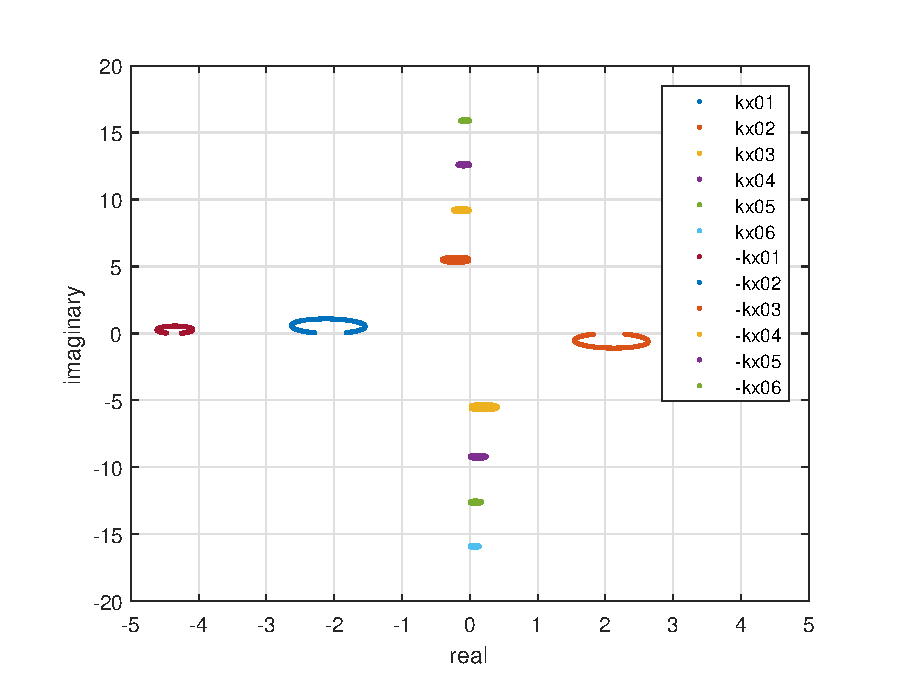
\includegraphics[width=1.13\linewidth]{kx01_20}
     \caption{$real(Z)=2$ and $im(Z)=-\infty \ to +\infty$}
    \end{subfigure}
    \caption{Axial wave numbers for $m=0,kR=4.353$ \cite{Kabral_thesis}}
\end{figure}
\noindent Cremer was the first to show the existence of a optimum radial wave number leading to the maximal axial decay rate of the least attenuate mode. This optimum condition correspond of the merging of two sequential order modes. For this specific condition the two modes collapse \cite{An_Introduction_to_Acoustics}.
\begin{figure}[H] \centering
    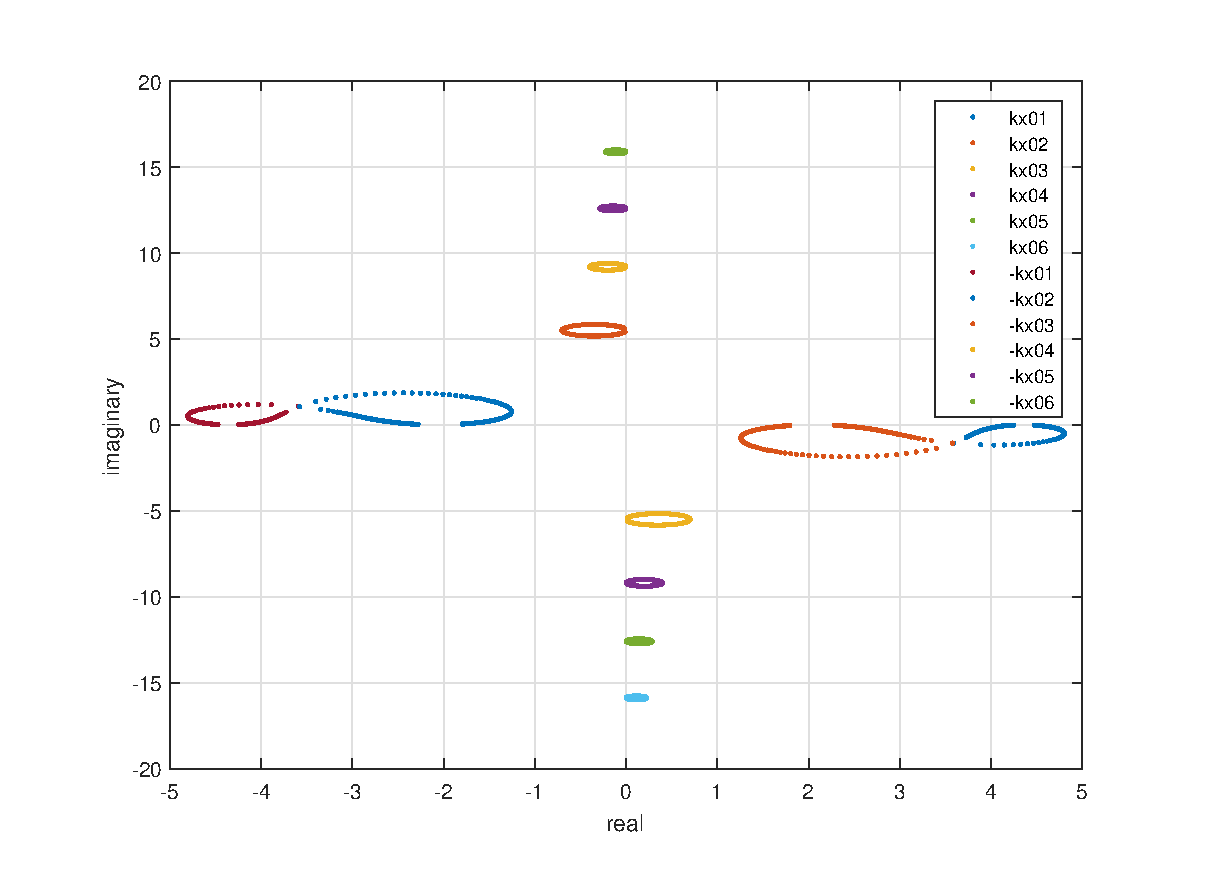
\includegraphics[scale=0.7]{kx01_Opt}
    \caption{Axial wave number in the complex plan for Im(Z) varying from -$\infty$ to +$\infty$\ and for Re(Z)=1.4165. For Im(Z)=-0.608 the first two modes coalesce $k_{01}=k_{02}=4.3-0.88i$ \cite{An_Introduction_to_Acoustics}}
\end{figure}
Cremer and Tester showed that this optimum wave number is given then the derived eigenvalue equation vanishes.
%------------------------------------------------------------------------------------------------------------
%------------------------------------------------------------------------------------------------------------
\subsubsection{Optimization of a circular liner}

The less attenuated mode has been found in an experimental setup and is the $(1,0)$ mode. To simplify the notation $k_r=k_{r,(1,0)}$ is used. The assumption of high frequency is made \cite{Kabral_thesis}: 
\begin{equation}
    k_x\approx\frac{k}{1\pm M_x}
\end{equation}
The eigenvalue for the $(1,0)$ mode is:
\begin{equation}
   \frac{ikR}{Z}=(1\pm M_x)^2 \frac{k_r r J_1^' (k_r r)}{J_1(k_r r)}
\end{equation}
The optimum radial wave number is:
\begin{equation}
    \frac{d}{dk_r r}\Bigg[(1\pm M_x)^2 \frac{k_r r J_1^' (k_r r)}{J_1(k_r r)}\Bigg]=0
\end{equation}
The equation is solved with the Matlab function "vpsolve". The optimum impedance determined is: 
\begin{equation}
    Z=   0.8918 - 0.3068i
\end{equation}
\begin{figure}[H] \centering
    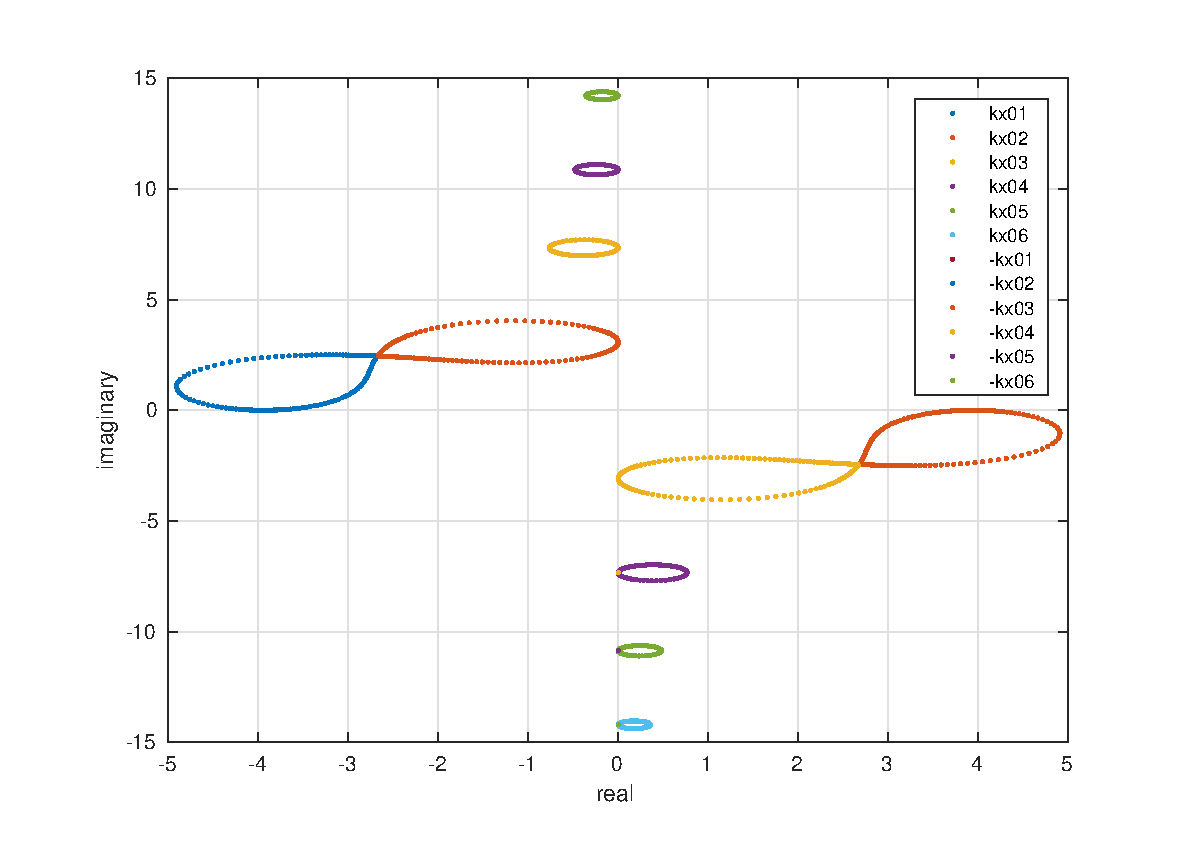
\includegraphics[scale=0.7]{kx11_OptCirc}
    \caption{Axial wave number in the complex plan for Im(Z) varying from -$\infty$ to +$\infty$\ and for Re(Z)=0.892. For Im(Z)=-0.307i the two modes coalesce $k_{11}=k_{12}=4.4663 + 1.467i$ \cite{An_Introduction_to_Acoustics}}
\end{figure}
%------------------------------------------------------------------------------------------------------------
%------------------------------------------------------------------------------------------------------------
\subsubsection{Optimization of an annular liner}
The optimization of an annular liner is more difficult and is rarely done by an analytically method. On the contrary with the circular duct, the eigenvalue solutions are not simple. The second problem is that the leass attenuate mode is rarely the plane wave mode. For our case, the leass attenuate mode was the $(8,0)$ and was determined by an experimental work. We tried to implement the Cremer impedance to reduce this mode.
The general solution of the pressure field for annular ducts is:
\begin{equation}
    p_{(m,n)}=\Big[A_{mn}J_m(k_{r,(m,n)}r)+B_{mn}Y_m(k_{r,(m,n)}r)\Big]\cos (m\theta) e^{i(\omega t-k_{x,(m,n)}x)}
\end{equation}
Where $J$ the Bessel function of the first type and order $m$ and $Y$ the Bessel function of the second type and order $m$.\\
From the general pressure solution and the Myers boundary conditions Eq.\eqref{eq:Myers}:
\begin{equation}
    ik\beta_1\Big[1-(\frac{k_{x,(m,n)}}{k})M\Big]^2=k_{r,(m,n)}\Bigg[\frac{A_{mn}J_m^'(k_{r,(m,n)}b)+B_{mn}Y_m^'(k_{r,(m,n)}b)}{A_{mn}J_m(k_{r,(m,n)}b)+B_{mn}Y_m(k_{r,(m,n)}b)}\Bigg]
\end{equation}
\begin{equation}
    ik\beta_0\Big[1-(\frac{k_{x,(m,n)}}{k})M\Big]^2=k_{r,(m,n)}\Bigg[\frac{A_{mn}J_m^'(k_{r,(m,n)}a)+B_{mn}Y_m^'(k_{r,(m,n)}a)}{A_{mn}J_m(k_{r,(m,n)}a)+B_{mn}Y_m(k_{r,(m,n)}a)}\Bigg]
\end{equation}
With $\beta$ the admittance of the inner and external wall (radius $b$ and $a$). For our application we choose to lined the external wall $\beta_1=0$ and the flow is zero $M=0$.\\
The eigenvalue equation follows:
\begin{equation}\label{CremerAnnular}
    ika\beta_0=-k_{r,(m,n)}a\Bigg(\frac{J_m^'(k_{r,(m,n)}a)Y_m^'(k_{r,(m,n)}b)-J_m^'(k_{r,(m,n)}b)Y_m^'(k_{r,(m,n)}a)}{J_m(k_{r,(m,n)}a)Y_m^'(k_{r,(m,n)}b)-J_m^'(k_{r,(m,n)}b)Y_m(k_{r,(m,n)}a)}\Bigg)
\end{equation}
We solve $\frac{d}{d(k_r)}\Big(Eq.\eqref{CremerAnnular}\Big)=0$ to find the optimum $k_{r,(m,n)}$. Then Eq.\eqref{CremerAnnular} is evaluated for this optimum wave number and gives the impedance.\\
The optimum impedance is: 
\begin{equation}
    Z=0.4537 + 0.0148i
\end{equation}\\
The eigenvalue equation has $n$ solutions. To attenuate the modes $(m,n)$, the first $m$ non zero solution has to be taken. The resolution is more detailed in \nameref{sec:AppendixB}.
\clearpage
